\documentclass[12pt]{article}
\usepackage[utf8]{inputenc}
\usepackage{graphicx}
\usepackage{amsmath}
\usepackage[margin=1in]{geometry}
\usepackage{indentfirst}
\usepackage{amsfonts}
%for english
\usepackage[portuguese]{babel}
%for portuguese
%\usepackage[portuguese]{babel}
\usepackage{float}
\usepackage[usenames,dvipsnames]{color}

\usepackage{listings}
\usepackage{color}

\definecolor{mygreen}{rgb}{0,0.6,0}
\definecolor{mygray}{rgb}{0.5,0.5,0.5}
\definecolor{mymauve}{rgb}{0.58,0,0.82}


\lstset{ %
  backgroundcolor=\color{white},   % choose the background color; you must add \usepackage{color} or \usepackage{xcolor}
  basicstyle=\footnotesize,        % the size of the fonts that are used for the code
  breakatwhitespace=false,         % sets if automatic breaks should only happen at whitespace
  breaklines=true,                 % sets automatic line breaking
  captionpos=b,                    % sets the caption-position to bottom
  commentstyle=\color{mygreen},    % comment style
  deletekeywords={...},            % if you want to delete keywords from the given language
  escapeinside={\%*}{*)},          % if you want to add LaTeX within your code
  extendedchars=true,              % lets you use non-ASCII characters; for 8-bits encodings only, does not work with UTF-8
  frame=single,                    % adds a frame around the code
  keepspaces=true,                 % keeps spaces in text, useful for keeping indentation of code (possibly needs columns=flexible)
  keywordstyle=\color{blue},       % keyword style
  language=C,                 % the language of the code
  morekeywords={*,...},            % if you want to add more keywords to the set
  numbers=left,                    % where to put the line-numbers; possible values are (none, left, right)
  numbersep=5pt,                   % how far the line-numbers are from the code
  numberstyle=\tiny\color{mygray}, % the style that is used for the line-numbers
  rulecolor=\color{black},         % if not set, the frame-color may be changed on line-breaks within not-black text (e.g. comments (green here))
  showspaces=false,                % show spaces everywhere adding particular underscores; it overrides 'showstringspaces'
  showstringspaces=false,          % underline spaces within strings only
  showtabs=false,                  % show tabs within strings adding particular underscores
  stepnumber=1,                    % the step between two line-numbers. If it's 1, each line will be numbered
  stringstyle=\color{mymauve},     % string literal style
  tabsize=2,                       % sets default tabsize to 2 spaces
  title=\lstname                   % show the filename of files included with \lstinputlisting; also try caption instead of title
}




\begin{document}
\renewcommand*\contentsname{Índice}

\begin{titlepage}

\newcommand{\HRule}{\rule{\linewidth}{0.5mm}} 
\center 
 

\textsc{\LARGE Universidade de Coimbra}\\[1.5cm] % Name of your university/college
\textsc{\Large Departamento de Engenharia Informática}\\[4cm] % Major heading such as course name
\textsc{\large Compiladores 2013/2014}\\[1cm] % Minor heading such as course title


\HRule \\[0.5cm]
{ \huge \bfseries Compilador para linguagem iJava}\\[0.4cm] 
\HRule \\[8cm]
 
\begin{minipage}{0.4\textwidth}
\begin{flushleft} \large
\emph{Autor:}\\
David \textsc{Cardoso}  \\Número: 2011164039
\end{flushleft}
\end{minipage}
~
\begin{minipage}{0.4\textwidth}

\begin{flushright} \large
\emph{Autor:} \\
Bruno \textsc{Caceiro}  \\Número: 2008107991
\end{flushright}
\end{minipage}\\[2cm]

{\large \today}\\[3cm]

\vfill

\end{titlepage}


\tableofcontents
\vfill
\pagebreak


\section{Introdução}
Este projecto consiste no desenvolvimento de um compilador para a linguagem \emph{iJava} (imperative Java), que consiste num pequeno subconjunto da linguagem Java (versão 5.0). Os programas da linguagem \emph{iJava} são constituídos por uma única classe (a principal), contendo necessariamente um método \emph{main}, e podendo conter outros métodos e atributos, todos eles estáticos e (possivelmente) públicos.

O projecto foi estruturado em 3 fases, primeiramente foi feita a Análise Lexical, implementada na linguagem \emph{C} e utilizando a ferramenta \emph{lex}. A segunda fase consistiu na análise sintática, recorrendo ao \emph{yacc/bison}, com a  construção da árvore de sintaxe abstrata e análise semântica (tabelas de símbolos, deteção de erros semânticos). No final foi feita a geração de código, em \emph{LLVM}.

\begin{figure}[H]
       \centering
       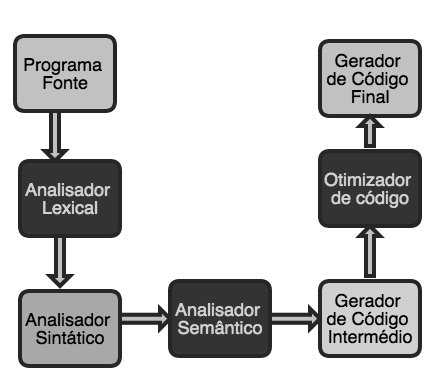
\includegraphics[keepaspectratio=true, width=300px]{fasesCompilacao.png}
       \caption{Fases de Compilação}
       \end{figure}

\pagebreak
\section{Análise Lexical}

A Análise Lexical consiste em analisar a entrada de linhas de caracteres e produzir uma sequência de símbolos (\emph{tokens}) que podem ser manipulados mais facilmente por um \emph{parser}. Assim, é uma forma de verificar um determinado alfabeto, neste caso o alfabeto da linguagem \emph{iJava}.
Esta análise pode ser dividida em três fases:
\begin{itemize}
	\item Extração e classificação de \emph{tokens};
	\item Eliminação de delimitadores e comentários;
	\item Tratamento de erros;
\end{itemize}


\subsection{Tokens}
\begin{itemize}
	        \item \textbf{ID:} Sequências alfanuméricas começadas por uma letra, onde os símbolos "\_" e "\$" contam como letras. Maiúsculas e minúsculas são consideradas ID's diferentes (\emph{case sensitive}).
	        \begin{itemize}
				\item \textbf{Expressão Regular}: $[a-zA-Z\_\$]([a-zA-Z\_\$0-9])* $
	        \end{itemize}
	         
	        \item \textbf{INTLIT:} Sequências de dígitos decimais e sequências de dígitos hexadecimais (incluindo a-f e A-F) precedidas de "0x"
	        \begin{itemize}
	        	\item \textbf{Expressão Regular:}  $(([0-9])+|("0x"[0-9a-$f$A-F]+))$  
	        \end{itemize}
	        \item \textbf{BOOLLIT:} "true" \text{\textbar} "false" 
	        \item \textbf{INT:} "int"
	        \item \textbf{BOOL:} "boolean"
	        \item \textbf{NEW:} "new"
	        \item \textbf{IF:} "if"
	        \item \textbf{ELSE:} "else"
	        \item \textbf{WHILE:} "while"
	        \item \textbf{PRINT:} "System.out.println"
	        \item \textbf{PARSEINT:} "Integer.parseInt"
	        \item \textbf{CLASS:} "class"
	        \item \textbf{PUBLIC:} "public"
	        \item \textbf{STATIC:} "static"
	        \item \textbf{VOID:} "void"
	        \item \textbf{STRING:} "String"
	        \item \textbf{DOTLENGTH:} ".length"
	        \item \textbf{RETURN:} "return"
	        \item \textbf{OCURV:} "("
	        \item \textbf{CCURV:} ")"
	        \item \textbf{OBRACE} "\{"
	        \item \textbf{CBRACE:} "\}"
	        \item \textbf{OSQUARE:} "["
	        \item \textbf{CSQUARE:} "]"	 
	        \item \textbf{ASSIGN:} "="
	        \item \textbf{SEMIC:} ";"
	        \item \textbf{COMMA:} ","
	      \end{itemize}
	      
	    Para a Análise Sintática foi necessário separar alguns \emph{tokens} devido às diferentes prioridades que cada operador tem. Assim, os \emph{tokens} foram agrupados pela ordem de precedência de operações.
		\begin{itemize}  
	        \item \textbf{OP1:} "\&\&"  
	        \item \textbf{OP1OR:} "\text{\textbar} \text{\textbar}"
	        \item \textbf{OP2:} "\textless" \text{\textbar} "\textgreater" \text{\textbar} "\textless=" \text{\textbar} "\textgreater="
	        \item \textbf{OP2EQS:} "==" \text{\textbar} "!="	        
	        \item \textbf{OP3:} "+" \text{\textbar} "-"
	        \item \textbf{OP4:} "*" \text{\textbar} "/" \text{\textbar} "\%"
	        \item \textbf{NOT:} "!"
	        \end{itemize}
	         O \emph{iJava} é um subconjunto da linguagem \emph{Java}, como tal, existe um conjunto de funcionalidades que embora não sejam suportadas, têm de ser consideradas. Assim, foi necessário tratar todo um conjunto de palavras reservadas de forma a permitir que sejam lexicalmente válidas mas não sintaticamente.
	         \begin{itemize} 
	        \item \textbf{RESERVED:}
	       	            \begin{itemize}
	       	                \item abstract
	       	                \text{\textbar} assert 
	       	                \text{\textbar} break 
	       	                \text{\textbar} byte 
	       	                \text{\textbar} case 
	       	                \text{\textbar} catch 
	       	                \text{\textbar} char 
	       	                \text{\textbar} const 
	       	                \text{\textbar} continue
	       	                 \text{\textbar} default 
	       	                 \text{\textbar} do 
	       	                 \text{\textbar} double
	       	                 \text{\textbar} enum 
	       	                 \text{\textbar} extends 
	       	                 \text{\textbar} final 
	       	                 \text{\textbar} finally 
	       	                 \text{\textbar} float 
	       	                 \text{\textbar} for 
	       	                 \text{\textbar} goto 
	       	                 \text{\textbar} implements 
	       	                 \text{\textbar} import 
	       	                 \text{\textbar} instanceof
	       	                 \text{\textbar} interface 
	       	                 \text{\textbar} long
	       	                 \text{\textbar} native
	       	                 \text{\textbar} package
	       	                 \text{\textbar} private 
	       	                 \text{\textbar} protected 
	       	                 \text{\textbar} short 
	       	                 \text{\textbar} strictfp
	       	                 \text{\textbar} super 
	       	                 \text{\textbar} switch 
	       	                 \text{\textbar} synchronized 
	       	                 \text{\textbar} this 
	       	                 \text{\textbar} throw 
	       	                 \text{\textbar} throws 
	       	                 \text{\textbar} transient 
	       	                 \text{\textbar} try
	       	                 \text{\textbar} volatile
		       	             \text{\textbar} null
	       	                 \text{\textbar} ++
	       	                 \text{\textbar} $--$
	       	            \end{itemize}      	 
		\end{itemize}
		
		\subsubsection{Comentários}
		Existem duas maneiras de fazer comentários:
		\begin{itemize}
			\item Comentar apenas uma linha "//\textless código\textgreater". \\Caso seja detectado (//)  todo o código que se segue é ignorado até encontrar uma mudança de linha.
			\subitem \textbf{Expressão Regular:} "//".*
			\item Comentar um bloco de código  "/*\textless código\textgreater */"
		\end{itemize} 
		\lstset{language=C,caption={Detecção de Comentários},label=Estruturas,frame=single}
		\begin{lstlisting}
		< COMMENT > <<EOF>> {BEGIN 0}
		< COMMENT > "*/"    {BEGIN 0}
		< COMMENT > "\n"    {}
		< COMMENT > .       {}
		"/*"	            {BEGIN COMMENT}
		\end{lstlisting}
		Caso seja detectado (/*) todo o código é ignorado até que seja encontrado o seu correspondente (*/). Caso seja detectado o EOF então é apresentada uma mensagem de erro: "Line \%d, col \%d: unterminated comment". Foi criado um estado adicional no \emph{lex} para poder tratar esta situação. Foi a criação deste estado que permitiu ignorar todos os \emph{tokens} presentes dentro do comentário.
		
		
		
		\subsubsection{Tratamento de Erros}
		Se forem detectados erros lexicais no ficheiro de entrada então é impressa uma mensagem de erro no \emph{stdout}:
		\begin{itemize}
            \item "Line\textless num linha\textgreater,col\textless num coluna\textgreater:illegal character('\textless c \textgreater'\textbackslash n)"
            \item "Line\textless num linha\textgreater,col\textless num coluna\textgreater:unterminated comment\textbackslash n"
        \end{itemize}
        \par Para podermos imprimir as mensagens de erro com o número da linha e coluna criámos uma variável \emph{column} para poder contar as colunas e utilizamos a variável \emph{yylineno},disponibilizada pelo \emph{yacc}, para sabermos o número das linhas.
        Para a contagem de colunas aumentamos a variável referente às colunas consoante o tamanho de cada \emph{token}. Quando há uma mudança de linha, inicializa-se o contador das colunas a 1. 
        \par Para tratar o caso dos comentários criámos duas variáveis adicionais (\emph{Commentline,Commentcolumn}) para poder guardar a coluna e linha onde o comentário é inicializado.
        
	
\pagebreak

\section{Análise Sintática e Semântica}
De forma a realizar a análise sintática foi utilizada a ferramenta \emph{lex}, para reconhecer e isolar os \emph{tokens}, sendo que de seguida serão enviados para o \emph{yacc} que irá ser responsável por verificar se estes pertencem à gramática da linguagem.


\begin{figure}[H]
       \centering
       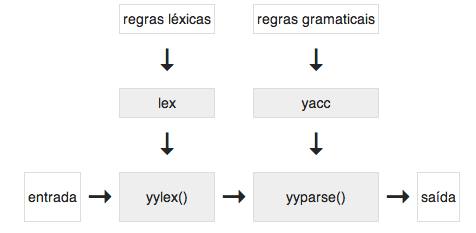
\includegraphics[keepaspectratio=true, scale = 0.82]{lex_yacc.png}
       \caption{Relacionamento entre \emph{lex} e \emph{yacc}, retirado de \emph{http://pt.wikipedia.org/wiki/Yacc}}
       \end{figure}
       
Para realizar a ligação entre o \emph{yacc} e o \emph{lex} foram definidos \emph{tokens} no  \emph{yacc},posteriormente importados pelo \emph{lex}. Sempre que o \emph{lex} detecta uma sequência de caracteres correspondente a um \emph{token} válido retorna um código acordado entre o \emph{yacc} e \emph{lex} de forma a identificar de forma única esse \emph{token} (\emph{enums}), sendo este valor enviado para o \emph{yacc}. 
Caso o \emph{token} corresponda a um tipo passível de ser processado (\emph{INTLIT, BOOLIT, ID e operadores}), é guardado na variável \emph{yyvar} o valor introduzido pelo utilizador.

\par Sendo a variável \emph{yylval} também responsável por definir o tipo de retorno de cada regra da gramática, foi necessário acrescentar outros tipos de dados, de forma a permitir a criação da árvore de sintaxe abstrata. Assim, foi criada uma \emph{union}, definida no \emph{yacc},que permite partilhar, no mesmo espaço de memória, vários tipos diferentes.

\lstset{language=c,caption={Union},label=Estruturas}
\begin{lstlisting}
%union{
    struct _Node* node;
    char* token;
    struct _idList* listId;
    int type;
}
\end{lstlisting}   

\par Para permitir a percepção, pelo \emph{yaac}, da linha e coluna que estão atualmente a serem utilizadas, foram também declaradas várias variáveis externas, partilhadas pelo \emph{lex}.
\lstset{language=c,caption=Variáveis externas,label=Estruturas2}
\begin{lstlisting}
extern int column;
extern int yylineno;
extern char* yytext;
extern int yyleng;
\end{lstlisting}  


\subsection{Gramática}

A gramática é a maneira formal de especificar a sintaxe de uma linguagem. 
Desenvolver uma gramática não ambígua é um dos passos mais importantes para o sucesso de um compilador. Para a gramática da linguagem \emph{iJava} usámos a notação \textbf{BNF} \emph{( Backus Naur Form)}, visto que a mesma é utilizada pelo \emph{yaac} e permite remover as ambiguidades. 


\subsubsection{Gramática Inicial}

\vspace{0.5cm}

\hspace{-1cm}Start $\rightarrow$ Program

\hspace{-1cm}Program $\rightarrow$ CLASS ID OBRACE { FieldDecl $\mid$ MethodDecl } CBRACE

\hspace{-1cm}FieldDecl $\rightarrow$ STATIC VarDecl

\hspace{-1cm}MethodDecl $\rightarrow$ PUBLIC STATIC ( Type $\mid$ VOID ) ID OCURV

[ FormalParams ] CCURV OBRACE { VarDecl } { Statement } CBRACE

\hspace{-1cm}FormalParams $\rightarrow$ Type ID { COMMA Type ID }

\hspace{-1cm}FormalParams $\rightarrow$ STRING OSQUARE CSQUARE ID

\hspace{-1cm}VarDecl $\rightarrow$ Type ID { COMMA ID } SEMIC

\hspace{-1cm}Type $\rightarrow$ ( INT $\mid$ BOOL ) [ OSQUARE CSQUARE ]

\hspace{-1cm}Statement $\rightarrow$ OBRACE { Statement } CBRACE

\hspace{-1cm}Statement $\rightarrow$ IF OCURV Expr CCURV Statement [ ELSE Statement ]

\hspace{-1cm}Statement $\rightarrow$ WHILE OCURV Expr CCURV Statement

\hspace{-1cm}Statement $\rightarrow$ PRINT OCURV Expr CCURV SEMIC

\hspace{-1cm}Statement $\rightarrow$ ID [ OSQUARE Expr CSQUARE ] ASSIGN Expr SEMIC

\hspace{-1cm}Statement $\rightarrow$ RETURN [ Expr ] SEMIC

\hspace{-1cm}Expr $\rightarrow$ Expr ( OP1 $\mid$ OP2 $\mid$ OP3 $\mid$ OP4 ) Expr

\hspace{-1cm}Expr $\rightarrow$ Expr OSQUARE Expr CSQUARE

\hspace{-1cm}Expr $\rightarrow$ ID $\mid$ INTLIT $\mid$ BOOLLIT

\hspace{-1cm}Expr $\rightarrow$ NEW ( INT $\mid$ BOOL ) OSQUARE Expr CSQUARE

\hspace{-1cm}Expr $\rightarrow$ OCURV Expr CCURV

\hspace{-1cm}Expr $\rightarrow$ Expr DOTLENGTH $\mid$ ( OP3 $\mid$ NOT ) Expr

\hspace{-1cm}Expr $\rightarrow$ PARSEINT OCURV ID OSQUARE Expr CSQUARE CCURV

\hspace{-1cm}Expr $\rightarrow$ ID OCURV [ Args ] CCURV

\hspace{-1cm}Args $\rightarrow$ Expr { COMMA Expr }

\vspace{0.5cm}

Lembramos que, em notação \textbf{ENBF}, os símbolos \textbf{[...]} englobam \emph{tokens} opcionais e \textbf{\{...\}} implicam a repetição dos \emph{tokens} 0 ou mais vezes.


\pagebreak
\subsubsection{Gramática Final}
\par A gramática que nos foi dada era ambígua e por isso tivemos de efetuar diversas alterações para permitir a análise sintática ascendente com o \emph{yacc}.\\
Algumas das alterações que efetuámos foram:
\begin{itemize}
	\item Criação de estados adicionais para as regras que implicam a repetição de \emph{tokens}.
	\item Criação de estados adicionais para as regras que continham \emph{tokens} opcionais
	\item Estabelecimento de regras de prioridade de forma a gerir regras de precedência entre operadores
	\item Definição das regras de associação dos operadores ( à esquerda/direita)
\end{itemize}

\lstset{language=c,caption=Associação de Operadores,label=Estruturas2}
\begin{lstlisting}
%nonassoc IFX
%nonassoc ELSE

%left OP1OR
%left OP1
%left OP2EQS
%left OP2
%left OP3
%left OP4
%right NOT
%left OSQUARE DOTLENGTH
\end{lstlisting}  


Apesar de termos usado recursividade  à direita, visto ser mais intuitiva, uma solução mais eficiente seria utilizar recursividade à esquerda, pois assim teríamos em memória apenas os elementos que estaríamos a analisar visto que estamos a efetuar reduções à medida que estamos a ler o \emph{input}.
\par Foram ainda necessárias realizar alterações na gramática, de forma a impedir a indexação de \emph{arrays} ($a[1][2]$). Para tal as expressões foram divididas em dois tipos, expressões indexáveis e não indexáveis.

$$$$

A gramática final, utilizada no \emph{yacc} é a seguinte apresentada.

\lstset{language=java,caption={Gramática Final},label=Estruturas,numbers=none, frame=none}
\begin{lstlisting}


Start :
            CLASS ID OBRACE field_or_method_declaration CBRACE;

field_or_method_declaration :
            FieldDecl field_or_method_declaration               
        |   MethodDecl field_or_method_declaration              
        | 
        ;

FieldDecl :
            STATIC VarDecl VarDecl_REPETITION;

MethodDecl :
            PUBLIC STATIC method_type_declaration ID OCURV FormalParams CCURV OBRACE VarDecl_REPETITION statement_declaration_REPETITION CBRACE;

method_type_declaration:
            Type            
        |   VOID            
        ;

FormalParams : 
            Type ID several_FormalParams        
        |   STRING OSQUARE CSQUARE ID           
        |                                           
        ;

several_FormalParams : 
            COMMA Type ID several_FormalParams      
        |                                               
        ;

VarDecl_REPETITION:
            VarDecl VarDecl_REPETITION      
         |                                      
         ;

VarDecl :
            Type ID several_var_decl_in_same_instructionOPTIONAL SEMIC;

several_var_decl_in_same_instructionOPTIONAL:
            COMMA ID several_var_decl_in_same_instructionOPTIONAL       
        |                                                                   
        ;

Type :
            INT OSQUARE CSQUARE        
       |    BOOL OSQUARE CSQUARE       
       |    INT                        
       |    BOOL                       
       ;
    

statement_declaration_REPETITION:
            Statement statement_declaration_REPETITION          
        |                                                           
        ;

Statement : 
            OBRACE several_statement CBRACE                     
        |   IF OCURV Expr CCURV Statement %prec IFX             
        |   IF OCURV Expr CCURV Statement ELSE Statement        
        |   WHILE OCURV Expr CCURV Statement                    
        |   PRINT OCURV Expr CCURV SEMIC                        
        |   ID array_indexOPTIONAL ASSIGN Expr SEMIC            
        |   RETURN return_expression SEMIC                      
        ;

several_statement:
            Statement several_statement     
        |                                       
        ;

array_indexOPTIONAL:
            OSQUARE Expr CSQUARE        
        |                                   
        ;

return_expression : 
            Expr    
        |               
        ;

IndexableExpr: 
            ID                                                  
        |   INTLIT                                              
        |   BOOLLIT                                             
        |   ID OCURV Args_OPTIONAL CCURV                        
        |   OCURV Expr CCURV                                    
        |   Expr DOTLENGTH                                      
        |   IndexableExpr OSQUARE Expr CSQUARE                  
        |   PARSEINT OCURV ID OSQUARE Expr CSQUARE CCURV        
        ;

Expr : 
            Expr OP1 Expr %prec OP1                 
        |   Expr OP1OR Expr %prec OP1OR             
        |   Expr OP4 Expr %prec OP4                 
        |   Expr OP3 Expr %prec OP3                 
        |   Expr OP2 Expr %prec OP2                 
        |   Expr OP2EQS Expr %prec OP2EQS           
        |   OP3 Expr %prec NOT                      
        |   NOT Expr %prec NOT                      
        |   NEW INT OSQUARE Expr CSQUARE            
        |   NEW BOOL OSQUARE Expr CSQUARE           
        |   IndexableExpr                           
        ;

Args_OPTIONAL:
            Args    
        |               
        ;

Args:
            Expr comma_expr;

comma_expr: 
            COMMA Expr comma_expr       
        |                                  
        ;
\end{lstlisting}
\subsection{Tratamento de Erros Sintáticos}
Para o tratamento de erros sintáticos utilizamos a função \emph{yyerror} que imprime a linha, a coluna e o input onde ocorreu o erro através da utilização das variáveis \emph{yylineno, column, yytext}. Assim, sempre que é detetado um erro um sintático é impressa uma mensagem de erro e terminada a execução do programa.

\lstset{language=c,caption=Função para tratamento erros sintáticos,label=Estruturas2,numbers=left,frame=single}
\begin{lstlisting}
void yyerror (char *var) {
		printf ("Line %d, col %d: %s: %s\n",yylineno,
           (int)(column-strlen(yytext)), var, yytext);
		Error = 1;
}
\end{lstlisting}  





\pagebreak
\subsection{Árvore de Sintaxe Abstrata}

\subsubsection{Estruturas}
Para a construção da árvore de sintaxe abstrata, optámos por utilizar um nó genérico (\emph{Node}) com a  seguinte estrutura: 

\lstset{language=C,caption={Estruturas para representação de Nós da Árvore},label=Estruturas,numbers=left,frame=single}
\begin{lstlisting}
/* General Node */
typedef struct _Node
{
    //Type of the Node (to identify the type of the node)
    NodeType n_type;

    //Type of the Struct (Int, Void, String,...)
    Type type;

    //Id or list of id's
    listID* id;

    //The Node's children (Method's/ Statements, Operators)
    struct _Node* n1;
    struct _Node* n2;
    struct _Node* n3;

    //Next node
    struct _Node* next;

    //Literals (to store the values)
    char* value;
	
	//Not used lololol
    char isStatic;
}Node;


/* Linked list of ID's (for multiple declaration of variables) */
typedef struct _idList
{
	//ID
	char* id;
	
	//Next ID
	struct _idList* next;
}listID;

\end{lstlisting}

Optámos por usar apenas uma única estrutura para representar toda a Árvore de Sintaxe Abstrata uma vez que qualquer nó poderia ser reduzido a um caso mais abstrato. Esta solução permitiu também que as operação realizadas sobre a árvore tenham sido simplificadas, visto não ser necessário realizar qualquer \emph{cast} ou conversão de tipo. Uma vez que a linguagem \emph{iJava} apresenta menos funcionalidades do que a linguagem \emph{Java}, foi possível optar por esta representação, mas tal poderia não se adaptar a um projeto mais complexo.


\lstset{language=C,caption={Identificadores únicos de cada \emph{Node}},label=Estruturas,numbers=left,frame=single}
\begin{lstlisting}
/* Type of the Node (to identify the type of the node) 
	- This enum allows us to uniquely identify each node and manipulate the data accordingly
*/
typedef enum {NODE_PROGRAM,
              NODE_VARDECL,
              NODE_METHODDECL,
              NODE_METHODPARAMS,
              NODE_METHODBODY,
              NODE_PARAMDECL,
              NODE_COMPOUNDSTAT,
              NODE_IFELSE,
              NODE_PRINT,
              NODE_RETURN,
              NODE_STORE,
              NODE_MUL,
              NODE_DIV,
              NODE_MOD,
              NODE_NOT,
              NODE_MINUS,
              NODE_PLUS,
              NODE_LENGTH,
              NODE_LOADARRAY,
              NODE_CALL,
              NODE_NEWINT,
              NODE_NEWBOOL,
              NODE_PARSEARGS,
              NODE_WHILE,
              NODE_STOREARRAY,
              NODE_INTLIT,
              NODE_BOOLLIT,
              NODE_ID,
              NODE_AND,
              NODE_OR,
              NODE_LESS,
              NODE_GREATER,
              NODE_LESSEQUAL,
              NODE_GREATEREQUAL,
              NODE_DIFFERENT,
              NODE_EQUAL,
              NODE_NULL,
              NODE_UNARYPLUS,
              NODE_UNARYMINUS,
              NODE_DONTPRINT
             } NodeType;
  
 /*Type of Node/Token (Int, Void, String,...) */            
typedef enum {TYPE_VOID, 
		       TYPE_INT,
		       TYPE_BOOL, 
		       TYPE_INT_ARRAY, 
		       TYPE_BOOL_ARRAY, 
		       TYPE_STRING_ARRAY
		       } Type;
\end{lstlisting}

 
 \subsubsection{Criação da Árvore}
\lstset{language=C,caption={Funções para a criação da árvore},label=Estruturas,numbers=left,frame=single} 
\begin{lstlisting}
/* Method to create an Id (a) */
listID* insertID(Node* currentNode, char* id);
/* Method to create a new VarId (int a,b,c (to link a to b to c)) */
listID* newVarID(char* id, listID* next);
/* Method to get an operator type (NODE_PLUS; NODE_NOT,...) */
NodeType getOperatorType(char* op);
/* Method to create a Null Node, used for mandatory child Nodes */
Node* createNull();
/* Method to create the Program itself (class gcd) */
Node* insertClass(char* id, Node* statements);
/* Method to create a new VarDecl (int a,b,c,d,e,f,g,h,i,j,k,l,m,n,o,p,q,r;)*/
Node* newVarDecl(int type, char* id, listID* moreIds, Node* next);
/* Method to link nodes */
Node* setNext(Node* current, Node* next);
/* Method to set a Node static */
Node* setStatic(Node* currentNode);
/* Creates a New Method Declaration Node: 
	public static void cenas(){statement1; statement2;return;} */
Node* newMethod(int type, char* id, Node* params, Node* varDecl, Node* statements);
/* Creates a Compound Node ({ expression1;expression2}) */
Node* insertCompound(Node* expression);
/* Creates an If node (if(true)) */
Node* insertIf(Node* expression, Node* statement1, Node* statement2);
/* Creates a Print Node (System.out.println("blica"))*/
Node* insertPrint(Node* expression);
/* Creates a While Node (while(true)) */
Node* insertWhile(Node* expression, Node* statements);
/* Creates a Return Node (return;  return true;)*/
Node* insertReturn(Node* expression);
/* Creates a Store Node (a = 5, b[5] = true) */
Node* insertStore(char* id, Node* arrayIndex, Node* expression);
/* Creates a Terminal Node (a, 5, true, false) */
Node* createTerminalNode(int n_type, char* token);
/* Creates a New Param Declaration Node (String[] argv, int a) */
Node* newParamDecl(int type, char* id, listID* moreIds, Node* next);
/* Creates a .length Node (argv.length) */
Node* insertDotLength(Node* expression);
/* Creates a Load Array Node (c[1]) */
Node* insertLoadArray(Node* expression, Node* indexExpression);
/* Creates a parse int Node (Integer.parseInt(argv[1])) */
Node* insertParseInt(char* id, Node* indexExpression);
/* Creates a new array Node (new int[1]) */
Node* insertNewArray(int type, Node* expression);
/* Creates a Method Call (teste(a,b)) */
Node* createCall(char* id, Node *args);
/* Creates an unary expression ( !true; -1;...)*/
Node* insertExpression(char* op,Node* exp);
/* Creates an binary expression  ( 1 + 1; true != false; a < b) */
Node* insertDoubleExpression(Node* exp1,char* op,Node* exp2);
 \end{lstlisting}

Para a criação da árvore é realizada pelo \emph{yacc} uma análise ascendente do \emph{input}, isto é, os nós vão sendo criados e agrupados de forma a representar a estrutura de cada regra gramatical. Assim, num primeira instância, são criados os nós terminais (declaração de variáveis, \emph{BOOLIT, INTLIT}) sendo posteriormente agrupados a operadores e expressões de forma a criar a estrutura do programa.

\subsubsection{Exemplo}
Considerando o seguinte programa:

\lstset{language=java,caption={Programa Exemplo},label=Estruturas,numbers=left,frame=single}
\begin{lstlisting}
 class gcd {
 	public static void main(String[] args) {
    	int x;
    	return;
	} 		
}
\end{lstlisting}

A árvore gerada é a seguinte:

\begin{figure}[H]
       \centering
       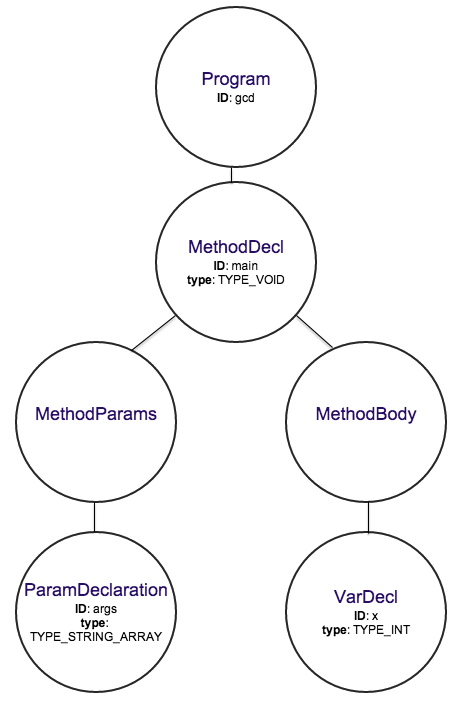
\includegraphics[keepaspectratio=true, scale = 0.5]{arvore.png}
       \caption{Árvore de Sintaxe Abstrata para o Programa Exemplo}
\end{figure}

 \subsubsection{Impressão da Árvore}
 Para imprimir a Árvore de Sintaxe Abstrata percorremos todos os nós 
 \lstset{language=c,caption={Funções para impressão da Árvore},label=Estruturas,numbers=left,frame=single}
 \begin{lstlisting}
 /* Method to print tabs */
 void printTabs(int i);
 /* Method to print the Syntax Abstract Tree */
 void printAST(Node* AST);
 /* Method to print the ID/ID's of the Node */
 void printIDs(listID* ids,int tabs, int n_type, int type);
 /* Recursive method to print the tree */
 void printSubTree(Node* currentNode, int tabs);
 \end{lstlisting}
 
 Para impressão da árvore de Sintaxe Abstrata tivémos em conta a indentação correta para cada Nó e utilizamos a estrutura auxiliar $NODE\_STRING[ ]$ onde guardamos a \emph{Node} que identifica cada tipo de \emph{Node}. Para tal, aproveitamos o facto do $NODE\_ID$ de cada nó ser parte uma enumeração, possibilitando assim que haja uma correspondência direta entre cada índice do array $NODE\_STRING[ ]$ e do $NODE\_ID$. 
 
\lstset{language=c,caption={Estrutura auxiliar para impressão da árvore},label=Estruturas,numbers=left,frame=single}
 \begin{lstlisting}
static const char *NODE_STRING[] = {"Program",
                 "VarDecl",
                 "MethodDecl",
                 "MethodParams",
                 "MethodBody",
                 "ParamDeclaration",
                 "CompoundStat",
                 "IfElse",
                 "Print",
                 "Return",
                 "Store",
                 "Mul",
                 "Div",
                 "Mod",
                 "Not",
                 "Sub",
                 "Add",
                 "Length",
                 "LoadArray",
                 "Call",
                 "NewInt",
                 "NewBool",
                 "ParseArgs",
                 "While",
                 "StoreArray",
                 "IntLit",
                 "BoolLit",
                 "Id",
                 "And",
                 "Or",
                 "Lt",
                 "Gt",
                 "Leq",
                 "Geq",
                 "Neq",
                 "Eq",
                 "Null",
                 "Plus",
                 "Minus",
                 "DON'T PRINT THIS!"
                 }; 
 \end{lstlisting} 
 


\subsection{Análise Semântica}
A Análise Semântica tem como principais objetivos a ligação das definições de variáveis com a sua utilização, a verificação da correção de tipos, declarações e chamadas de funções.
Esta análise é dividida em duas fases:
	\begin{enumerate}
		\item Processar as declarações de variáveis e métodos:
		\begin{itemize}
			\item Adicionar novas entradas na tabela de símbolos
			\item Apresentar mensagem de erro caso haja \emph{Ids} repetidos
		\end{itemize}
		\item Processar os \emph{statements}
		\begin{itemize}
			\item Verificar se as variáveis utilizadas foram declaradas no  \emph{scope} local (do método) ou no \emph{scope} global, e em caso de variável não declarada, apresentar mensagem de erro
			\item Usar a tabela de símbolos para determinar o tipo de cada expressão e procurar erros de concordância de tipo (atribuições, cálculos, contagem e tipos de argumentos corretos,...)
		\end{itemize}
	\end{enumerate}

\subsection{Tabela de Símbolos}

A Tabela de símbolos é criada a partir da Árvore de Sintaxe Abstrata, onde se percorrem todos os nós relativos às declarações de métodos e atributos. Assim é criada uma tabela para cada \emph{scope},ou seja uma tabela global do programa e uma para cada método.
 
\subsubsection{Estruturas}
Para representação da tabela de símbolos, foram utilizadas as seguintes estruturas:
\lstset{language=C,caption={Estruturas para representação da Tabela de Símbolos},label=Estruturas,frame=single}
\begin{lstlisting}
/* Table Node */
typedef struct _TableNode
{
    //Type of the Node (to identify the type of the node)
    TableType n_type;
    
    //Type of the Struct (Int, Void, String,...)
    Type type;
    
    //ID or list of id's
    listID* id;
    
    //Next node
    struct _TableNode* next;
    
    //If is a param
    char isParam;
}TableNode;

/* Table */
typedef struct _Table{
    TableNode* table;
    struct _Table* next;
}Table;

\end{lstlisting}

\subsubsection{Criação da Tabela de Símbolos}

Durante a criação da tabela de símbolos é realizada a verificação da existência de IDs duplicados dentro do mesmo \emph{scope}.

\lstset{language=C,caption={Métodos para criação da Tabela de Símbolos},label=Estruturas,frame=single}
\begin{lstlisting}
/* Method to add a variable declaration to a scope  */
TableNode* addNewDeclTable(char isparam, TableNode* symbol, Node* ast,
												    	Table* table);
/* Goes through the AST and creates the scopes  adding the Method's and Variables */												    	
Table* createSymbols(Node* ast);
\end{lstlisting}

\subsubsection{Impressão da Tabela de Símbolos}
Tal como ocorreu com a Árvore de Sintaxe Abstrata foi utilizado um \emph{array} de \emph{Strings} para fazer a correspondência entre $NODE\_ID$ e o \emph{output} esperado. Neste \emph{array} no entanto foi necessário uma especial atenção ao fato do \emph{output} esperado ser exatamente o \emph{input} do utilizador e não o \emph{token} de cada nó.

\lstset{language=C,caption={Funções impressão da tabela de símbolos},label=Estruturas,frame=single}
\begin{lstlisting}
/* Goes through the tables, prints the header and calls printSymbolsDecl method */
void printSymbols(Table* table);
/* Prints the declarations of each table */
void printSymbolsDecl(TableNode* tableNode);

static const char *OPERATOR_STRING[] = {"Program",
                 "VarDecl",
                 "MethodDecl",
                 "MethodParams",
                 "MethodBody",
                 "ParamDeclaration",
                 "CompoundStat",
                 "if",
                 "System.out.println",
                 "return",
                 "=",
                 "*",
                 "/",
                 "%",
                 "!",
                 "-",
                 "+",
                 ".length",
                 "[",
                 "call",
                 "new int",
                 "new boolean",
                 "Integer.parseInt",
                 "while",
                 "=",
                 "IntLit",
                 "BoolLit",
                 "Id",
                 "&&",
                 "||",
                 "<",
                 ">",
                 "<=",
                 ">=",
                 "!=",
                 "==",
                 "null",
                 "+",
                 "-"
                 };

\end{lstlisting}

\pagebreak
\subsection{Tratamento de Erros Semânticos}
Para o tratamento de erros semânticos utilizamos as seguintes funções:
\lstset{language=C,caption={Funções para tratamento de erros semânticos},label=Estruturas,frame=single}
\begin{lstlisting}
/*Check if ID is already declared in the scope */
void   checkIfExists(char* id, Table* local);
/* Check if ID exists:
	- If exists return the Type 
	- If doesn't exist, print error message: "Cannot find symbol %s\n" and exit 
*/
int    checkifIDExists(char* id,TableType type, Table* table, Table* main);
/* Check if the Literal is valid (decimal / hexadecimal / octal)
	- If it is invalid print error message: "Invalid literal %s\n" and exit
*/
void   validIntLit(char* lit);
/*goes through the AST and check for errors in every node */
void   checkSemanticErrors(Node* ast, Table* local, Table* main);
/*check if terminal nodes are correct*/
void   checkErrors(Node* ast, Table* symbols, Table* main);
/*check if the types of the operators are correct, and propagates those types through the tree*/
void   checkTypes(Node* ast,Table* main);
/*Gets the local scope */
Table* getMethodTable(Table* main, char* methodID);
/* Get the type of the function */
int    getFunctionType();
/* Get the name of the function */
char*  getFunctionName();
/*Change to another scope */
void   setTable(Table * oi);

/* Prints the correspondent error */
void   operatorError2Types(int op,int n1, int n2);
void   operatorError1Types(int op,int n1);
void   assignmentError(char* var, int n1, int n2);
void   assignmentErrorArray(char* var, int n1, int n2);
void   statementError(int op, int n1,int n2);
void   statementError1oranother(int op, int n1, int n2, int n3);
void   getErrorCall(int i,char* name, int n1, int n2);

\end{lstlisting}

Na detecção de erros semânticos foi realizada a verificação da consistência entre os símbolos terminais e operadores.
\par Um dos problemas com que nos deparámos durante a verificação de erros foi a adequação da mensagem de erro ao nó onde ocorre o erro. Tal facto levou a que, apesar de todas as funcionalidades estarem implementadas, não fosse possível concluir a meta 2 atempadamente, embora os erros fossem apenas de \emph{output} ("\emph{presentation error}"). 
\par Foi necessária especial atenção com alguns tipos de nós como o $NODE\_CALL$ uma vez que era necessária realizar a verificação de todos os seus parâmetros, o $NODE\_LENGTH$ e $NODE\_PARSEARGS$ uma vez que poderiam utilizar \emph{Strings}.Nos restantes nós foi necessário verificar os tipos dos nós filhos bem como o tipo resultante da aplicação do operador. Assim, durante a verificação semântica propagamos os tipos de forma a que todos os nós guardem o tipo de retorno.



\pagebreak
\section{Geração de Código}

Para a realização da geração de código foi necessário ter em conta certos aspetos, nomeadamente os parâmetros e tipo de retorno da função \emph{main}, uma função obrigatória em \emph{iJava} e em \emph{LLVM}. Assim foi necessário permitir a recepção de parâmetros no formato definido pelo \emph{ANSI-C} ($int$ $main(int$ $argc,$ $char** argv$)).
\par Outro aspecto a ter em conta foi a necessidade de armazenar a dimensão dos \emph{arrays} alocados em memória. Para tal, foi criada uma estrutura, de forma a permitir o armazenamento de dois valores, o espaço de memória alocado e o tamanho desse espaço.
\par Além disso, tivemos de ter em consideração o \emph{Short Circuiting}, ou seja, o segundo argumento é apenas executado ou avaliado se o primeiro argumento não for suficiente para determinar o valor da expressão: quando o primeiro argumento de uma função $AND$ é avaliado como falso, o valor global deve ser falso e quando o primeiro argumento da função $OR$ for avaliado como verdadeiro, o valor global deve ser verdadeiro. Para realizar estes requisitos, recorremos à utilização de saltos condicionais.
\par Outro aspecto a considerar, foi a necessidade de garantir que todas as funções apresentassem um chamada de retorno. Para não ser necessária a utilização de saltos condicionais, decidimos acrescentar sempre no final de cada função uma expressão de retorno, mesmo que a mesma não possa ser alcançada.
\par Por fim, foi necessário  criar variáveis locais para armazenar os parâmetros, que são passados por valor e por isso não eram passíveis de ser acedidos da mesma forma que outras variáveis.
\par Devido ao facto de a árvore de sintaxe abstrata já conter os tipos de dados devolvidos pelos operadores, foi-nos possível gerar a maioria o código sem a necessidade de utilizar a tabela de símbolos, sendo que apenas a utilizamos para verificar a origem das variáveis (globais ou locais).





\lstset{language=C,caption={Função e estrutura auxiliar},label=Estruturas,frame=single}
\begin{lstlisting}
char* generateCode(Node* ast,Table* main);

typedef struct _callP{
    Type type;
    char name[100];
    struct _callP* next;
}callParams;
\end{lstlisting}

\lstset{language=C,caption={Tamanho de dados e operadores},label=Estruturas,frame=single}
\begin{lstlisting}
static const char* SYMBOLS_TYPE_SIZE[] = {     "void",     "i32",     "i1",
"%.ArrayInt",     "%.ArrayBool",     "i8*",     "Id",     "i32",
"i1",     "i1*",  };

static const char *CODE_OPERATOR_STRING[] = {"Program",
                 "VarDecl",
                 "MethodDecl",
                 "MethodParams",
                 "MethodBody",
                 "ParamDeclaration",
                 "CompoundStat",
                 "if",
                 "System.out.println",
                 "return",
                 "=",
                 "mul",
                 "sdiv",
                 "srem",
                 "!",
                 "sub",
                 "add",
                 ".length",
                 "[",
                 "call",
                 "new int",
                 "new boolean",
                 "Integer.parseInt",
                 "while",
                 "=",
                 "IntLit",
                 "BoolLit",
                 "Id",
                 "and",
                 "or",
                 "slt",
                 "sgt",
                 "sle",
                 "sge",
                 "ne",
                 "eq",
                 "null",
                 "+",
                 "-"
                 };
\end{lstlisting}



\end{document}